\documentclass[border=8pt]{standalone}
\usepackage[T1]{fontenc}\usepackage{helvet}\renewcommand{\familydefault}{\sfdefault}
\usepackage{tikz}\usetikzlibrary{arrows.meta, positioning, calc, backgrounds}
\definecolor{ink}{HTML}{1a1916}
\definecolor{inktwo}{HTML}{3a3a35}
\definecolor{inkthree}{HTML}{6a6862}
\definecolor{rule}{HTML}{b8b09a}
\definecolor{amber}{HTML}{a8730a}
\definecolor{red}{HTML}{c8261a}
\definecolor{paper}{HTML}{f0eee5}
\definecolor{slab}{HTML}{d8d4c6}
\tikzset{
  >={Stealth[length=2.2mm]},
  wire/.style={line width=0.8pt, ink},
  modwire/.style={line width=0.6pt, dashed, ink},
  tastewire/.style={line width=0.6pt, dashed, amber},
  gatewire/.style={line width=0.6pt, dotted, ink},
  block/.style={rectangle, draw=ink, line width=0.9pt, fill=slab, minimum width=3.0cm, minimum height=1.9cm, inner sep=0pt},
  perf/.style={rectangle, draw=ink, line width=0.7pt, minimum width=3.0cm, minimum height=0.7cm, inner sep=2pt, font=\footnotesize, text=ink},
  title/.style={font=\scriptsize\bfseries, text=ink, anchor=north, inner sep=2pt},
  jack/.style={circle, draw=ink, fill=paper, line width=0.5pt, minimum size=3.2pt, inner sep=0pt},
  plabel/.style={font=\tiny, text=inktwo, anchor=west, inner sep=1pt},
  olabel/.style={font=\tiny, text=inktwo, anchor=east, inner sep=1pt},
  settings/.style={font=\scriptsize, text=ink, align=left, anchor=north west, inner sep=1pt, text width=2.9cm},
}
\begin{document}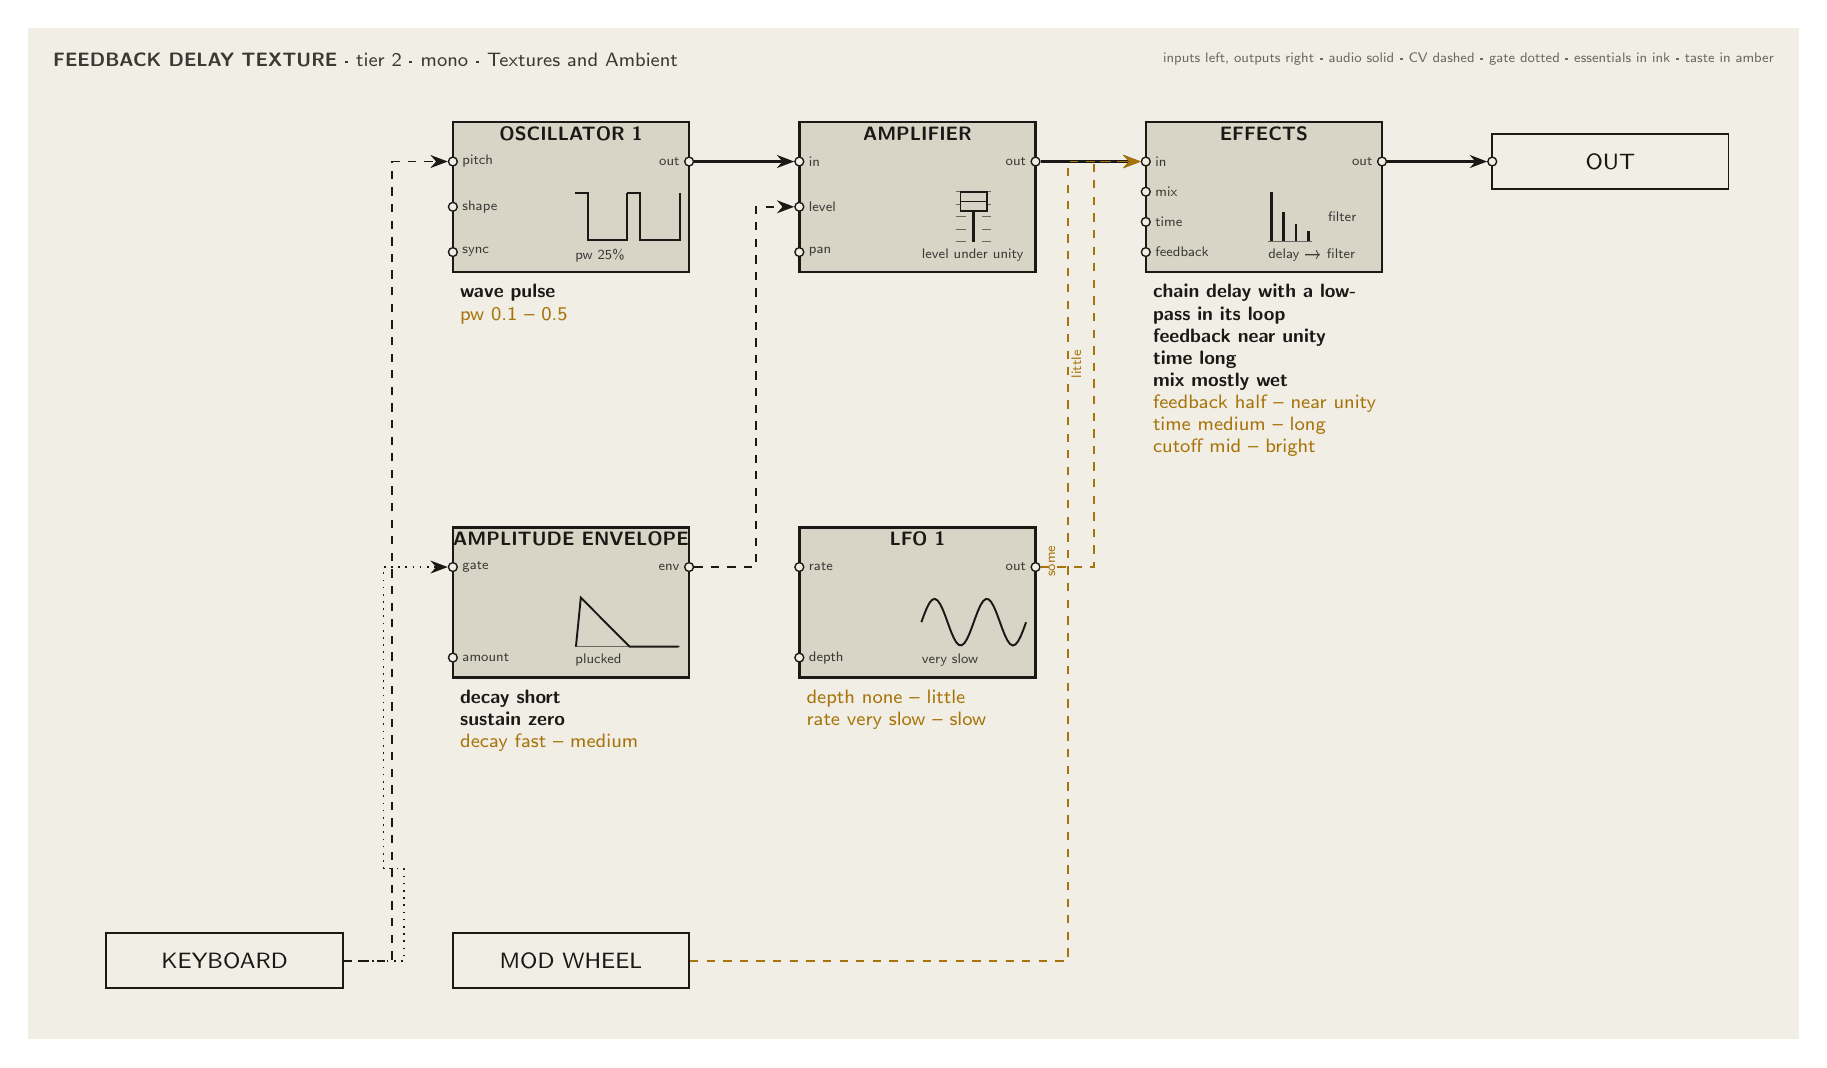
\begin{tikzpicture}
\begin{scope}[on background layer]\fill[paper] (-2.5,-10.7) rectangle (20.0,2.15);\end{scope}
\node[block, minimum height=1.9cm] (osc1) at (4.4,0.0) {};
\node[title] at (osc1.north) {OSCILLATOR 1};
\node[jack] (osc1-pitch) at (2.9000000000000004,0.44999999999999996) {};
\node[plabel] at (2.9800000000000004,0.44999999999999996) {pitch};
\node[jack] (osc1-shape) at (2.9000000000000004,-0.125) {};
\node[plabel] at (2.9800000000000004,-0.125) {shape};
\node[jack] (osc1-sync) at (2.9000000000000004,-0.7) {};
\node[plabel] at (2.9800000000000004,-0.7) {sync};
\node[jack] (osc1-out) at (5.9,0.44999999999999996) {};
\node[olabel] at (5.82,0.44999999999999996) {out};
\begin{scope}
\draw[ink, line width=0.7pt] (4.450,0.046) -- (4.616,0.046) -- (4.616,-0.546) -- (5.115,-0.546) -- (5.115,0.046);
\draw[ink, line width=0.7pt] (5.115,0.046) -- (5.281,0.046) -- (5.281,-0.546) -- (5.780,-0.546) -- (5.780,0.046);
\node[font=\tiny, text=inktwo, anchor=north west, inner sep=0pt] at (4.450,-0.650) {pw 25\%};
\end{scope}
\node[settings] at (2.95,-1.0699999999999998) {\textbf{wave pulse} \\ \textcolor{amber}{pw 0.1 -- 0.5}};
\node[block, minimum height=1.9cm] (amp) at (8.8,0.0) {};
\node[title] at (amp.north) {AMPLIFIER};
\node[jack] (amp-in) at (7.300000000000001,0.44999999999999996) {};
\node[plabel] at (7.380000000000001,0.44999999999999996) {in};
\node[jack] (amp-level) at (7.300000000000001,-0.125) {};
\node[plabel] at (7.380000000000001,-0.125) {level};
\node[jack] (amp-pan) at (7.300000000000001,-0.7) {};
\node[plabel] at (7.380000000000001,-0.7) {pan};
\node[jack] (amp-out) at (10.3,0.44999999999999996) {};
\node[olabel] at (10.22,0.44999999999999996) {out};
\begin{scope}
\draw[ink, line width=1.2pt] (9.515,-0.570) -- (9.515,0.070);
\draw[inkthree, line width=0.3pt] (9.295,-0.570) -- (9.415,-0.570) (9.615,-0.570) -- (9.735,-0.570);
\draw[inkthree, line width=0.3pt] (9.295,-0.410) -- (9.415,-0.410) (9.615,-0.410) -- (9.735,-0.410);
\draw[inkthree, line width=0.3pt] (9.295,-0.250) -- (9.415,-0.250) (9.615,-0.250) -- (9.735,-0.250);
\draw[inkthree, line width=0.3pt] (9.295,-0.090) -- (9.415,-0.090) (9.615,-0.090) -- (9.735,-0.090);
\draw[inkthree, line width=0.3pt] (9.295,0.070) -- (9.415,0.070) (9.615,0.070) -- (9.735,0.070);
\fill[slab, draw=ink, line width=0.6pt] (9.345,-0.178) rectangle (9.685,0.062);
\draw[ink, line width=0.5pt] (9.345,-0.058) -- (9.685,-0.058);
\node[font=\tiny, text=inktwo, anchor=north west, inner sep=0pt] at (8.850,-0.650) {level under unity};
\end{scope}
\node[block, minimum height=1.9cm] (fx) at (13.200000000000001,0.0) {};
\node[title] at (fx.north) {EFFECTS};
\node[jack] (fx-in) at (11.700000000000001,0.44999999999999996) {};
\node[plabel] at (11.780000000000001,0.44999999999999996) {in};
\node[jack] (fx-mix) at (11.700000000000001,0.06666666666666665) {};
\node[plabel] at (11.780000000000001,0.06666666666666665) {mix};
\node[jack] (fx-time) at (11.700000000000001,-0.31666666666666665) {};
\node[plabel] at (11.780000000000001,-0.31666666666666665) {time};
\node[jack] (fx-feedback) at (11.700000000000001,-0.7) {};
\node[plabel] at (11.780000000000001,-0.7) {feedback};
\node[jack] (fx-out) at (14.700000000000001,0.44999999999999996) {};
\node[olabel] at (14.620000000000001,0.44999999999999996) {out};
\begin{scope}
\draw[inkthree, line width=0.3pt] (13.250,-0.561) -- (13.809,-0.561);
\draw[ink, line width=0.9pt] (13.295,-0.561) -- (13.295,0.061);
\draw[ink, line width=0.9pt] (13.451,-0.561) -- (13.451,-0.188);
\draw[ink, line width=0.9pt] (13.608,-0.561) -- (13.608,-0.337);
\draw[ink, line width=0.9pt] (13.764,-0.561) -- (13.764,-0.427);
\node[font=\tiny, text=inktwo] at (14.194,-0.250) {filter};
\node[font=\tiny, text=inktwo, anchor=north west, inner sep=0pt] at (13.250,-0.650) {delay → filter};
\end{scope}
\node[settings] at (11.750000000000002,-1.0699999999999998) {\textbf{chain delay with a low-pass in its loop} \\ \textbf{feedback near unity} \\ \textbf{time long} \\ \textbf{mix mostly wet} \\ \textcolor{amber}{feedback half -- near unity} \\ \textcolor{amber}{time medium -- long} \\ \textcolor{amber}{cutoff mid -- bright}};
\node[block, minimum height=1.9cm] (aenv) at (4.4,-5.1499999999999995) {};
\node[title] at (aenv.north) {AMPLITUDE ENVELOPE};
\node[jack] (aenv-gate) at (2.9000000000000004,-4.699999999999999) {};
\node[plabel] at (2.9800000000000004,-4.699999999999999) {gate};
\node[jack] (aenv-amount) at (2.9000000000000004,-5.85) {};
\node[plabel] at (2.9800000000000004,-5.85) {amount};
\node[jack] (aenv-out) at (5.9,-4.699999999999999) {};
\node[olabel] at (5.82,-4.699999999999999) {env};
\begin{scope}
\draw[inkthree, line width=0.3pt] (4.450,-5.711) -- (5.780,-5.711);
\draw[ink, line width=0.7pt] (4.463,-5.711) -- (4.525,-5.089) -- (5.146,-5.711) -- (5.146,-5.711) -- (5.767,-5.711);
\node[font=\tiny, text=inktwo, anchor=north west, inner sep=0pt] at (4.450,-5.800) {plucked};
\end{scope}
\node[settings] at (2.95,-6.22) {\textbf{decay short} \\ \textbf{sustain zero} \\ \textcolor{amber}{decay fast -- medium}};
\node[block, minimum height=1.9cm] (lfo1) at (8.8,-5.1499999999999995) {};
\node[title] at (lfo1.north) {LFO 1};
\node[jack] (lfo1-rate) at (7.300000000000001,-4.699999999999999) {};
\node[plabel] at (7.380000000000001,-4.699999999999999) {rate};
\node[jack] (lfo1-depth) at (7.300000000000001,-5.85) {};
\node[plabel] at (7.380000000000001,-5.85) {depth};
\node[jack] (lfo1-out) at (10.3,-4.699999999999999) {};
\node[olabel] at (10.22,-4.699999999999999) {out};
\begin{scope}
\draw[ink, line width=0.7pt] plot[domain=0:1, samples=40, variable=\u] ({8.850+\u*1.330},{-5.770+(0.740)*(0.5+0.4*sin(360*\u*2))});
\node[font=\tiny, text=inktwo, anchor=north west, inner sep=0pt] at (8.850,-5.800) {very slow};
\end{scope}
\node[settings] at (7.3500000000000005,-6.22) {\textcolor{amber}{depth none -- little} \\ \textcolor{amber}{rate very slow -- slow}};
\node[perf] (key) at (0.0,-9.7) {KEYBOARD};
\node[perf] (wheel) at (4.4,-9.7) {MOD WHEEL};
\node[perf, fill=paper] (out) at (17.6,0.44999999999999996) {OUT}; \node[jack] (out-in) at (16.1,0.44999999999999996) {};
\draw[wire,->] (osc1-out) -- (amp-in);
\draw[wire,->] (amp-out) -- (fx-in);
\draw[wire,->] (fx-out) -- (out-in);
\draw[modwire,->] (aenv-out) -- (6.750000000000001,-4.699999999999999) -- (6.750000000000001,-0.125) -- (amp-level);
\draw[tastewire,->] (lfo1-out) -- (11.040000000000001,-4.699999999999999) -- (11.040000000000001,0.44999999999999996) -- (fx-in);
\node[font=\tiny, text=amber, anchor=south, inner sep=1pt, rotate=90] at (10.920000000000002,-2.1249999999999996) {little};
\draw[modwire,->] (key.east) -- (2.1300000000000003,-9.7) -- (2.1300000000000003,0.44999999999999996) -- (osc1-pitch);
\draw[gatewire,->] (key.east) -- (2.28,-9.7) -- (2.28,-8.53) -- (2.0200000000000005,-8.53) -- (2.0200000000000005,-4.699999999999999) -- (aenv-gate);
\draw[tastewire,->] (wheel.east) -- (10.71,-9.7) -- (10.71,0.44999999999999996) -- (fx-in);
\node[font=\tiny, text=amber, anchor=south, inner sep=1pt, rotate=90] at (10.590000000000002,-4.625) {some};
\node[anchor=north west, font=\scriptsize, text=inktwo] at (-2.3,1.95) {\textbf{FEEDBACK DELAY TEXTURE} · tier 2 · mono · Textures and Ambient};
\node[anchor=north east, font=\tiny, text=inkthree] at (19.8,1.95) {inputs left, outputs right · audio solid · CV dashed · gate dotted · essentials in ink · taste in amber};
\end{tikzpicture}\end{document}
